\section{Support for Large Number of Streams Using Internal Streams}


\subsection{I/O activity with large lifetime variance}
For most PCs, their lifetime distributions tend to have small variances.  
However, we observed that a few outlier PCs which have large lifetime variations. 
For example, when multiple I/O contexts are covered by the same write system function, 
the corresponding PC may represent several I/O contexts whose data lifetimes are quite different.   
Such a case occurs, for example, 
in the compaction module of RocksDB.
RocksDB maintains
several levels, L1, ..., L$n$, in the persistent storage, except for L0 (or a
memtable) stored in DRAM.  Once one level, say L2, becomes full, all the data
in L2 is compacted to a lower level, i.e., L3.  It involves moving data from L2
to L3, along with the deletion of the old data in L2.  In the
LSM tree~\cite{LSM}, a higher level is smaller than a lower level 
(i.e., the size of (L2) $<$ the size of (L3)). 
Thus, data stored in a higher level is invalidated more frequently than those kept
in lower levels, thereby having shorter lifetimes.

In order to mitigate the side effect of a few outlier PCs with large lifetime variances, 
we use internal streams based on a two-phase stream assignment technique.

%Once the L1 becomes full,
%\textit{all} the data kept in the L1 are moved to the L2 by the compaction
%module.  The same operation is applied to the other levels (i.e., L3, ...,
%L$n-1$).  The compaction involves reading and writing data from a higher level
%(e.g., L1) to a lower level (e.g., L2).  The data in a higher level (e.g., L1)
%is then removed.  

%While the program context can be used as a useful indicator that determines the
%lifetime of data, we also observe that the same PC could generate data 
%with diverged lifetimes. One of the representative examples is the compaction
%module of RocksDB. RocksDB maintains several levels, L1, ..., L$n$, in the
%persistent storage, except for L0 (or a memtable) stored in DRAM.  Data flushed
%from the memtable are first written to the L1.  Once the L1 becomes full,
%\textit{all} the data kept in the L1 are moved to the L2 by the compaction
%module.  The same operation is applied to the other levels (i.e., L3, ...,
%L$n-1$).  The compaction involves reading and writing data from a higher level
%(e.g., L1) to a lower level (e.g., L2).  The data in a higher level (e.g., L1)
%is then removed.  In the LSM-tree, a higher level is smaller than a lower
%level. Thus, data stored in a higher level is invalidated sooner than data kept
%in lower levels, thereby having much shorter lifetimes.

Unfortunately, in the current RocksDB implementation, the compaction step is supported 
by the same execution path (i.e., the same PC) regardless of the level.
Therefore, the PC for the compaction activity cannot effectively separate data with 
short lifetimes from one with long lifetimes.
Fig.~\ref{fig:compaction}(a) shows 
the lifetime distribution collected from the compaction-activity PC.  
Since this distribution includes lifetimes of data written from all the levels, 
its variance is large.  
When we manually separate the single compaction step into several per-level compaction steps, 
as shown in Figs. 5(b) and 5(c), the lifetime distributions of per-level compaction steps 
show smaller variances.   
In particular, L2 and L3 show distinct lifetime distributions from that of L4.
Data from L2 and L3 are likely to have shorter lifetimes, while L4 has generally
long-lived data as shown in Fig. 5(d).

\begin{figure}[!t]
\centering
%\vspace{-7pt}
\hfill
\subfloat[compaction: all levels]{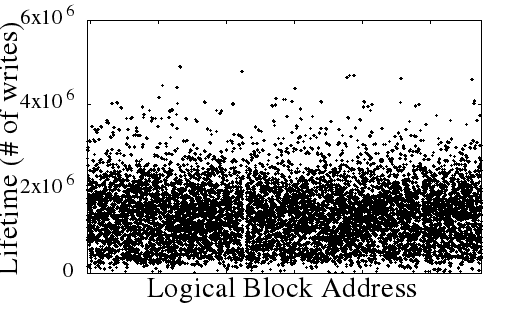
\includegraphics[width=0.19\textwidth]{figure/pc_3}}
	\hspace{2pt}
\subfloat[compaction: L2]{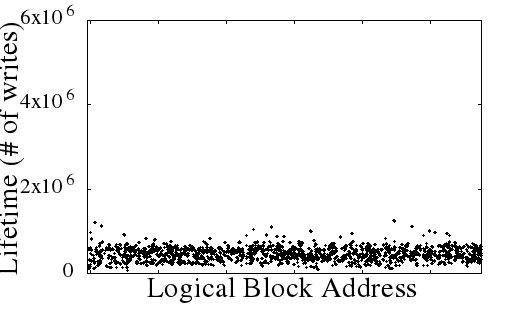
\includegraphics[width=0.19\textwidth]{figure/type_4}}  % data from 4/03040047
\hfill
\vspace{-1pt}
\subfloat[compaction: L3]{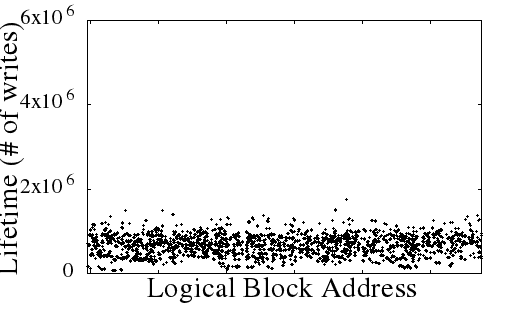
\includegraphics[width=0.19\textwidth]{figure/type_5}}
	\hspace{2pt}
\subfloat[compaction: L4]{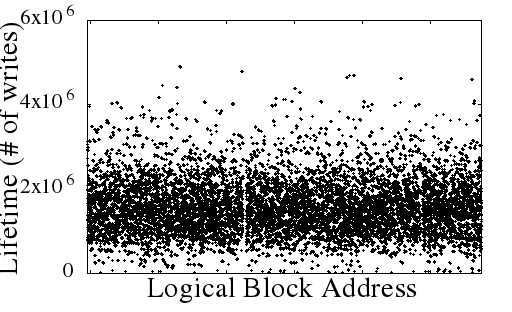
\includegraphics[width=0.19\textwidth]{figure/type_6}}
%\vspace{-10pt}
%\caption{The lifetime distribution of the compaction activity.} 
\caption{Lifetime distributions of the compaction activity at different levels.} %shane part
\label{fig:compaction}
%\vspace{-20pt}
\end{figure}

\subsection{Low resource requirement of internal streams}

In Section 2.2, we describe various resource overheads that limit the number of external streams.
In the case of an internal stream used for internal data migration of SSD, 
it has a relatively small resource overhead due to its distinguishing characteristics from the external stream
and it can be used to manage the lifetime variance within streams.

Unlike external streams, which require host requests to be handled directly in the foreground,
internal streams can be handled as background operations, 
so even if the data structures of internal streams are located in relatively slow memory, 
performance may not suffer. 
Under saturated conditions, which require concurrent processing of GC while processing a host write request, performance degradation may occur if slower memory is used in the internal stream, but performance degradation is small compared to using slow memory for external streams.

With regard to power resources, the buffering mechanism can be used for internal streams to maximize flash parallelism, but there is a big difference that no power resource is required to guarantee data integrity of buffered data.
Buffered data of host write will be lost if the data is not stored during power off handling.
However, the buffered data of internal migration doesn't need to be saved during power off handling. Because the original data always exists in the source block of migration. Therefore, there is no problem in ensuring data integrity without special handling or power resource requirement.

The increase of the active point for data migration has the same problem that WAF might be increased by reducing the overprovision area. However, in most workloads, when multiple active points are used for the internal stream, it helps to better manage the lifetime variations within the stream, thereby reducing overall WAF.

\subsection{Internal Streams: Separating long-lived data during GC}
Since it is difficult to separate data with different lifetimes within the same PC 
(as in the compaction-activity PC), we devised a two-phase method that decides SSD 
streams in two levels: the main stream ID in a host level and the internal stream ID in an SSD level.
Conceptually, long-lived data in the main stream are moved to its internal stream to 
separate from (future) short-lived data of the main stream.
Although moving data to the internal stream may increase WAF,
the overhead can be hidden if we restrict the internal stream move during GC only.
Since long-lived data (i.e., valid pages) in a victim block are moved to a free block during GC, 
they can be moved to the internal stream by changing the target block.
For instance, \textsf{\small PCStream} assigns the compaction-activity PC {\it pID} to a
main stream {\it sID} for the first phase.
To separate the long-lived data of {\it pID} (e.g., L4 data) 
from future short-lived data of {\it pID} (e.g., L1 data), 
valid pages of the {\it sID} are assigned to its internal stream for the second phase during GC.



